%!TEX TS-program = xelatex
%!TEX encoding = UTF-8 Unicode

% Kod treba da se sredi (beautify-je)
% i malo jos da se optimizuje, da se
% uklone upozorenja i slicno 

\documentclass[a4paper, 11pt]{article}
\usepackage[bindingoffset=0mm,%
            left=19mm,right=19mm,top=30mm,bottom=20mm,%
	    footskip=12mm]{geometry}
	   
\usepackage[english]{babel}
\usepackage[utf8]{inputenc}
\usepackage[parfill]{parskip}	    
\usepackage{indentfirst}
\setlength{\parindent}{0cm}
\usepackage[T1]{fontenc}
\usepackage{graphicx}
\graphicspath{ {img/} }
\usepackage{wrapfig}
\addto\captionsenglish{\renewcommand{\figurename}{\textbf{Slika}}}

\usepackage{paralist}
\usepackage{amsmath}
\usepackage{relsize}
\usepackage{amsfonts}
\usepackage{listings}
\usepackage{xcolor}
\usepackage[shortlabels]{enumitem}
\usepackage{xltxtra,fontspec,xunicode}
\setmonofont[Scale=1,Ligatures=NoCommon]{Inconsolata}

% No Spacing Itemize
\usepackage{paralist}
  \let\itemize\compactitem
  \let\enditemize\endcompactitem
  \let\enumerate\compactenum
  \let\endenumerate\endcompactenum
  \let\description\compactdesc
  \let\enddescription\endcompactdesc
  \pltopsep=\medskipamount
  \plitemsep=1pt
  \plparsep=1pt

\lstset{basicstyle=\scriptsize\ttfamily,breaklines=true}
% \lstset{framextopmargin=10pt,framexbottommargin=10pt, frame=lines}
%\lstset{lineskip={-0.5pt}}

\lstset {
  language=C,
  backgroundcolor=\color{lightgray!20},
  captionpos=0, % sets the caption-position to bottom
  %belowcaptionskip=1\baselineskip,
  breaklines=true,
  xleftmargin=\parindent,
  tabsize=6, % sets default tabsize to 2 spaces
  showstringspaces=false,
  basicstyle=\footnotesize\ttfamily,
  keywordstyle=\bfseries\color{blue!65},
  commentstyle=\itshape\color{green!55!black},
  identifierstyle=\color{black},
  stringstyle=\color{orange!85!black},
  framextopmargin=2pt,
  %framexleftmargin=1,
  %framexrightmargin=1,
  framexbottommargin=2pt,
  frame=single, % adds a frame around the code
  rulecolor=\color{gray!65!black}
  }

  \lstset{
	language=customc,
	keywords=[2]{EXIT_FAILURE,false,MAP_FAILED},
	keywords=[3]{AST_STD, AST_PER, NULL},
	keywords=[4]{include},
	keywords=[5]{<stdio.h>},
	keywords=[6]{EXIT_SUCCESS,true},
	keywords=[7]{STDIN_FILENO, STDOUT_FILENO,BUF_SIZE,BUF_MAX,MAX_LEN, 
	SIGINT,SIGKILL,SIGSTOP,F_OK,SIG_ERR,SIG_IGN,READ_SIDE,WRITE_SIDE, O_RDONLY,
	O_WRONLY,O_RDWR,O_NONBLOCK,O_CREAT,PROT_READ,PROT_WRITE,MAP_SHARED,F_WRLCK,
	F_RDLCK,SEEK_SET,F_SETLK,F_UNLCK},	
	keywordstyle=[2]{\color{red!60!black}},
	keywordstyle=[3]{\color{cyan!85!black}},
	keywordstyle=[4]{\color{brown}},
	keywordstyle=[5]{\color{brown}},
	keywordstyle=[6]{\color{green!55!black}},
	keywordstyle=[7]{\color{magenta!80!black}},
	morecomment=[l][\color{magenta!80!black}]{\#},
	otherkeywords={pid_t,off_t}
	%otherkeywords={define,\# }
  }

\usepackage[framemethod=TikZ]{mdframed}

\usepackage{hyperref}
\hypersetup{
    colorlinks,
    citecolor=black,
    filecolor=black,
    linkcolor=black,
    urlcolor=black
}

\usepackage{titling}
\setlength{\droptitle}{38mm}  

\newcommand{\scode}[3] {
	\hspace{.06\textwidth} 
	\begin{minipage}[t]{.88\textwidth} % Width (ex. .475)
		\begin{mdframed}[topline=true,bottomline=true,leftline=true,rightline=true,backgroundcolor=gray!22, linecolor=gray!60!black,roundcorner=1mm]
			\lstinputlisting[caption="", label=lst:#3, language=customc]{/home/kotur/Documents/LaTeX/Projects/OS/primeri/#1} 

	\begin{center}
		\caption{\textbf{Primer \ref{lst:#3}:} #2}
	\end{center}
	\end{mdframed}
	\end{minipage}

}

\newcommand{\stdio}[4] {
	\hspace{.06\textwidth} 
	\begin{minipage}[t]{.88\textwidth} % Width (ex. .475)
		\begin{mdframed}[backgroundcolor=black!7,topline=true,bottomline=true,leftline=true,rightline=true,roundcorner=1mm]
		\begin{minipage}[t]{.5\textwidth} % Width (ex. .475)
			\textbf{#1} \\
				\texttt{#3}
		\end{minipage}
		\begin{minipage}[t]{.5\textwidth} % Width (ex. .475)
			\textbf{#2} \\
				\texttt{#4}
		\end{minipage}
		\end{mdframed}
	\end{minipage}
	\vspace{3mm} 
}

\usepackage{fancyhdr}

\pagestyle{fancy}
\renewcommand{\subsectionmark}[1]{\markboth{#1}{}} % set the \leftmark
\fancyhf{}
\fancyhead[R]{\texttt{\thepage}} % predefined ()
\fancyhead[L]{\texttt{\leftmark}} % 1. sectionname
\fancyfoot[C]{}
\fancypagestyle{plain}{%
  \fancyhf{}%
  \renewcommand{\headrulewidth}{0pt}%
}
\setlength{\headsep}{6mm}

\usepackage{tikz}
\usetikzlibrary{calc}
\newcommand\HRule{\rule{\textwidth}{1pt}}

\begin{document}

\begin{titlepage}

%            NASLOV                         PODNASLOV                  AUTOR ...
	\title{\textbf{\texttt{\textcolor{blue!50!cyan!70!black}{Operativni sistemi}}} \\ \vspace{1mm} \large{\texttt{\textcolor{blue!50!cyan!70!black}{podsetnik za praktični deo ispita}}}}
	\author{\texttt{\textcolor{blue!50!cyan!70!black}{github.com/kotur95}}}
	\date{\vspace{-2mm}\small{\texttt{\color{blue!50!cyan!70!black}{26.08.2017.}}}}

\maketitle
\begin{tikzpicture}[remember picture, overlay, color=blue!50!cyan!40!white]
  \draw[line width = 32pt] ($(current page.north west) + (0cm,-0cm)$) rectangle ($(current page.south east) + (-0cm,0cm)$);
\end{tikzpicture}

\begin{center}
	\vspace{5mm} 
	
\includegraphics[width=.7\textwidth]{Gnulove.png}
\end{center}
\thispagestyle{empty}
\end{titlepage} 

\thispagestyle{empty}
\newpage~\newpage


% TABLE OF CONTENTS
\renewcommand{\contentsname}{\LARGE{Sadržaj}}
\tableofcontents
\thispagestyle{empty}
\setcounter{page}{2}
\newpage

\pagestyle{fancy}

\section{Obrada grešaka}

\subsection{Funkcije za obradu grešaka}

Funkcija \texttt{ast()} služi za obradu grešaka nastalih u sistemskim pozivima, tačnije ukoliko data greška modifikuje \texttt{errno} promenljivu \texttt{<errno.h>}. 

Funkcija \texttt{err\_check()} obrađuje standardne grešaka koje mogu nastati tokom izvrsavanja programa.

Funkcija \texttt{pth\_check()} služi za obradu gresaka kod funkcija koje rade sa posix threadovima.

\scode{ast.c}{Funkcije za obradu grešaka}{obrg}
\vspace{2mm} 

\vspace{2mm} 
Primer poziva funkcije za obradu greske prilikom open sistemskog poziva: \\

\begin{center}
\vspace{-5mm} 
	\texttt{ast((fd = open(fpath, O\_RDONLY)), "Greska prilikom otvaranja fajla za citanje");} 
\end{center}
Primer poziva funkcije za proveru broja argumenata bio bi: \\

\begin{center}
\vspace{-5mm} 
\texttt{err\_check(argc == 2, "Greska - program prima 2 argumenta");} 
\end{center}
Primer poziva funkcije za obradu greske prilikom poziva funkcije \texttt{pthread\_create()} bio bi: \\

	\begin{center}
		\vspace{-5mm} 
		\texttt{pth\_check(pthread\_create(thread\_id, NULL, thr\_func, args), "Error creating thread");}
	\end{center}

	\vspace{1mm} 

Funkcije date u Primeru \ref{lst:obrg} biće korišćene u narednim primerima.

\newpage

\subsection{Primeri obrade grešaka.}

U ovoj sekciji biće predstavljeni primeri upotrebe funkcija za obradu gresaka.

\subsubsection{Pogrešan broj argumenata}

\scode{wnarg.c}{Pogresan broj argumenata}{wnarg}

\subsubsection{Otvaranje regularnog fajla}

U Primeru \ref{lst:otvorobr} možemo videti primer gde se ograđujemo od raznih grešaka prilikom otvaranja fajla.

\scode{openerchk.c}{Otvaranje regularnog fajla}{otvorobr}
\vspace{2mm} 

\texttt{access(file, F\_OK)} --- proverava da li fajl uopšte postoji. Slično možemo pokušati da vidimo da li nam je fajl dostupan za čitanje/pisanje promenom drugog argumenta u \texttt{R\_OK} ili \texttt{W\_OK}.

Izraz na osnovu kojeg je kreirana provera da li je fajl regularan \texttt{(sbuf.st\_mode \& S\_IFMT) == S\_IFREG)} se može pronaći u man strani za \texttt{stat()} funkciju: \texttt{man 2 stat}.

\subsubsection{Kreiranje niti}

\scode{pthcrer.c}{Obrada greske za funkcije koje rade sa threadovima}{pthcrer}


 
%In the middle if you want to change the margins use
%\newgeometry{left=0.8in,right=0.8in,top=1in,bottom=1in} 

\newpage

\section{Praktični primeri}

\subsection{Obrada signala}

Signal je obaveštenje procesu da je neki događaj nastupio. Tip signala se određuje u zavisnosti od vrednosti signala, u tom smislu signal je određen celobrojnom promenljivom pomoću koje se identidikuje. Funkcije i signalne promenljie (identifikatori) se nalaze u zaglavlju \texttt{<signal.h>}. Signali se nekada opisuju kao \emph{hardware interupt-s} jer su analogni njima, tj. prekidaju normalan tok izvršavanja programa. U većini slučajeva nije moguće predvideti kada će neki signal nastupiti.

Postoje takozvane uobičajene reakcije na signal koji je poslat procesu, i njih možemo videti u man strani za signal sistemski poziv (\texttt{man 2 signal}).   

Signal sistemski poziv prima 2 argumenta, prvi argument je celobrojna vrednost signala predstavljena simboličkim imenom koje možemo naći u \texttt{man 2 signal}, drugi argument je \texttt{signal handler} funkcija koja obrađuje taj, a ponekad i više signala,\texttt{signal handler} prima jedan argument a to je redni broj \texttt{signal-a} koji je nastupio. Ukoliko ne želimo da menjamo uobičajeno ponačanje kao drugi argument \texttt{signal()} sistemskog poziva prosleđujemo vrednost \texttt{SIG\_DFL}, a ukoliko želimo da zanemarimo signal \texttt{SIG\_IGN}. 

\begin{center}
	\texttt{void (*signal(int sig, void (*func)(int)))(int);}
\end{center}

\textbf{Povratna vrednost:} Ukoliko je signal obrađen, povratna vrednost je ista kao povratna vrednost \texttt{signal handler-a}, za poslednji signal tog tipa. Ukoliko je došlo do greške povratna vrednost je \texttt{SIG\_ERR} i \texttt{errno} promenljiva je postavljena na odgovarajuću vrednost.

\scode{signals.c}{Obrada signala}{signals}

\newpage
\subsection{Kreiranje deteta}

Funkcija \texttt{fork()} kreira novi proces duplirajući proces iz kojeg je pozvana. Novi proces je dete procesa iz kojeg je \texttt{fork()} funkcija pozvana. Oba procesa imaju zaseban memorijski prostor sa istim sadržajem, i međusobno ne dele memoriju.

\vspace{2mm} 
\begin{figure}[h]
	\centering
	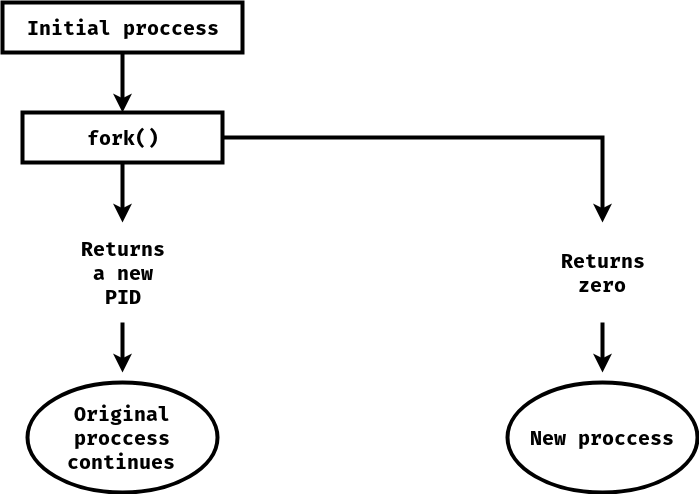
\includegraphics[width=.48\textwidth]{fsc.png} % size, path
	\caption{Fork sistemski poziv}
	\label{fig:fsc}
\end{figure}
\vspace{2mm} 

Dete je identičan duplikat roditelja, ali neke stvari ne nasleđuje:
\vspace{-3mm} 
\begin{enumerate}[1)]
	\item{\texttt{PID-ovi} su im različiti.}
	\item{\texttt{PID} roditelja ostaje nepromenjen.}
	\item{Dete ne nasleđuje \texttt{lock-ove} memorije roditelja.}
	 \item{Dete ne nasleđuje izmene semafora od roditelja.}
	 \item[]{itd ...}
\end{enumerate}

Prototip funkcije je: \texttt{pid\_t fork(void);} \\

\vspace{-6mm} 

\textbf{Povratna vrednost:} \texttt{PID} deteta roditelju i 0 detetu. U slučaju greške funkcija vraća \texttt{-1} roditelju i dete ne biva kreirano. Vrednost \texttt{errno} promenljive se postavlja na odgovarajucu vrednost.

\scode{fork.c}{Fork poziv}{fork}
\stdio{Standardni ulaz:}{Standardni izlaz:}{}{Hello from parent, pid: 7896 \\ Hello from child, pid: 0}

% U Primeru \ref{lst:fork} vidimo kako \texttt{fork()} funkcija kreira dete i dodeljuje mu segment u kodu. 
% \texttt{PID} roditeljskog procesa u detetu možemo dobiti pozivanjem funkcije:
% \begin{center}
% 	\texttt{pid\_t getppid(void);} 
% \end{center}

\newpage

\subsection{Exec familija funkcija}

U \texttt{unix-olikim} operativnim sistemima zamena tekućeg procesa nekim drugim procesom (programom) se vrši pomoću \texttt{exec()} familije sistemskih poziva. Ovaj metod se najčešće koristi u kombinaciji sa \texttt{fork()} sistemskim pozivom, u kome se dete procesa zamenuje nekim drugim procesom (programom). 

Sistemski pozivi koji pripadaju \texttt{exec()} familiji:

\hspace{.15\textwidth} 
\begin{minipage}[t]{.7\textwidth} % Width (ex. .475)
	\begin{verbatim}
	       int execl(const char *path, const char *arg, ...
			       /* (char  *) NULL */);
	       int execlp(const char *file, const char *arg, ...
			       /* (char  *) NULL */);
	       int execle(const char *path, const char *arg, ...
			       /*, (char *) NULL, char * const envp[] */);
	       int execv(const char *path, char *const argv[]);
	       int execvp(const char *file, char *const argv[]);
	       int execvpe(const char *file, char *const argv[],
			       char *const envp[]);
       \end{verbatim}
\end{minipage}

Prvi argument kod ovih funkcija predstavlja ime izvršnog fajla koji će biti pokrenut kao zamena trenutne slike procesa. Funkcije \texttt{execlp(), execvp(), i execvpe()} šta više ne zahtevaju tačnu putanju do programa, tj. ukoliko je prvi argument bez vodeće \texttt{/} date funkcije tragaju za izvršnim fajlom u direktorijumu koji je uključen u \texttt{PATH} enviroment promenljivoj \texttt{shell} programa.
	
Postoje sledeće varijacije \texttt{exec()} sistemskog poziva u odnosu na sufiks, od kojih zavisi drugi argument.

\begin{itemize}[]
	\item{\texttt{'p'} - Funkcija uzima \texttt{filename} i koristi \texttt{PATH} da nađe izvršni fajl.}
	\item{\texttt{'l'} - Funkcija uzima listu argumenata umesto pokazivača.}
	\item{\texttt{'v'} - Argument je vektor \texttt{argv[]}}
	\item{\texttt{'e'} - Funkcija uzima \texttt{envp[]} niz umesto trenutnog \texttt{enviroment-a}}
\end{itemize}

\textbf{Povratna vrednost:} Nema povratka u slučaju uspeha, \texttt{-1} u slucaju greške - \texttt{errno} promenljiva se postavlja na odgovarajuću vrednost.

\vspace{-1mm} 
\scode{exec.c}{Exec sistemski poziv}{exec}

\vspace{2mm} 
Rezultat rad programa iz \ref{lst:exec} je ispisivanje informacija o tekućem folderu na standardni izlaz, kao prilikom komande \texttt{shell-a: \$ ls -l}.

\newpage
\subsection{Pravljenje PIPE-a}
Funkcija \texttt{pipe()} kreira pipe, kao argument prima niz tipa \texttt{int} dužine 2, i dodeljuje mu vrednosti fajl deskriptora koje je otvorila. Fajlovi na koje referišu ti fajl deskriptori su (\texttt{pipefd[0]}) tj. strana \texttt{pipe-a} za čitanje i (\texttt{pipefd[1]}) strana \texttt{pipe-a} za pisanje.  
\begin{center}
	\texttt{int pipe(int fildes[2]);}
\end{center}

\textbf{Povratna vrednost:} \texttt{0} u slučaju uspešnog kreiranja \texttt{pipe-a}, \texttt{-1} u slucaju greške.

\texttt{PIPE} je struktura koja omogućava jednosmernu komunikaciju, dat je primer \texttt{pipe-a} u shell programu: 

\begin{center}
	\texttt{\$ ls | wc -l}  
\end{center}

Ova komanda ispisuje broj fajlova u tekućem direktorijumu, tako što izlaz programa \texttt{ls} postaje ulaz programa \texttt{wc} koji potom obrađuje taj ulaz i štampa na standardni izlaz broj linija (fajlova).
U sledećem primeru pokučaćemo da prikažedmo jednu od implementacija ovog \texttt{PIPE-a}.

\scode{pipe.c}{Pipe (ls | wc -l) izmedju roditelja i deteta}{pipewc}
\vspace{3mm} 

Dakle rezultat rada programa iz Primera \ref{lst:pipewc} je ispisuje broja fajlova u direktorijumu iz kog je pokrenut.
\newpage

\begin{figure}[h]
	\centering
	\vspace{3mm} 
	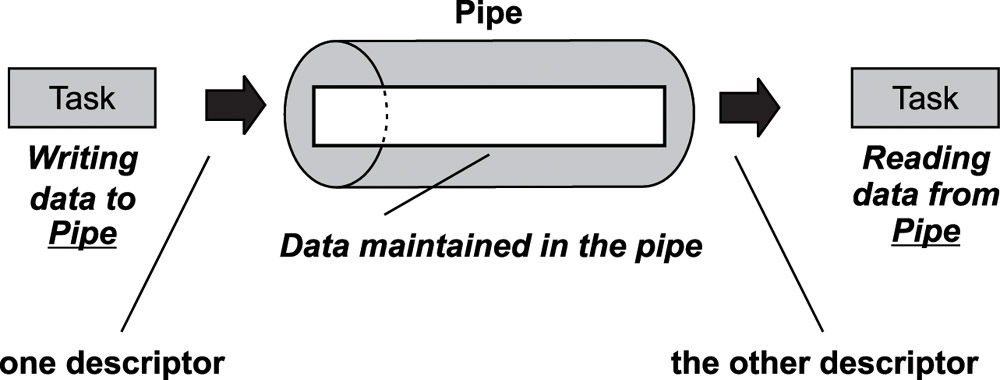
\includegraphics[width=.65\textwidth]{pipe.jpg} % size, path
	\caption{Komunikacija putem PIPE-a}
	\label{fig:lpipe}
\end{figure}

\subsection{Jednosmerna komunikacija između procesa (FIFO)}

\texttt{FIFO} je varijacija \texttt{PIPE} koncepta, \texttt{FIFO} se definiše kao \texttt{byte stream} što znači da se ne može podacima pristupiti u proizvoljnom redosledu, već onako kako oni putuju kroz \texttt{FIFO}. \texttt{PIPE} nam je omogućio komunikaciju između roditeljskog procesa i deteta, dok nam \texttt{FIFO} omogućuje komunikaciju između 2 ``nepovezana" procesa. Otvaranje \texttt{FIFO-a} je slično kao kod regularnog fajla, i \texttt{PIPE-a}. 

Fifo se može kreirati na dva načina:
\vspace{-2mm} 
\begin{enumerate}[1)]
	\item{shell komandom: \texttt{mkfifo [-m mode] pathname}}
	\item{sistemskim pozivom: \texttt{mkfifo()}}
\end{enumerate}

Nakon kreiranja \texttt{FIFO} se otvara \texttt{open()} sistemskim pozivom, ali sa flag-ovima: \texttt{O\_RDONLY} ili \texttt{O\_WRONLY}, jer se koristi za komunikaciju u jednom smeru. Može ga otvoriti svaki proces, ako ima odgovarajuće privilegije.

\vspace{1mm} 
\begin{figure}[h]
	\centering
	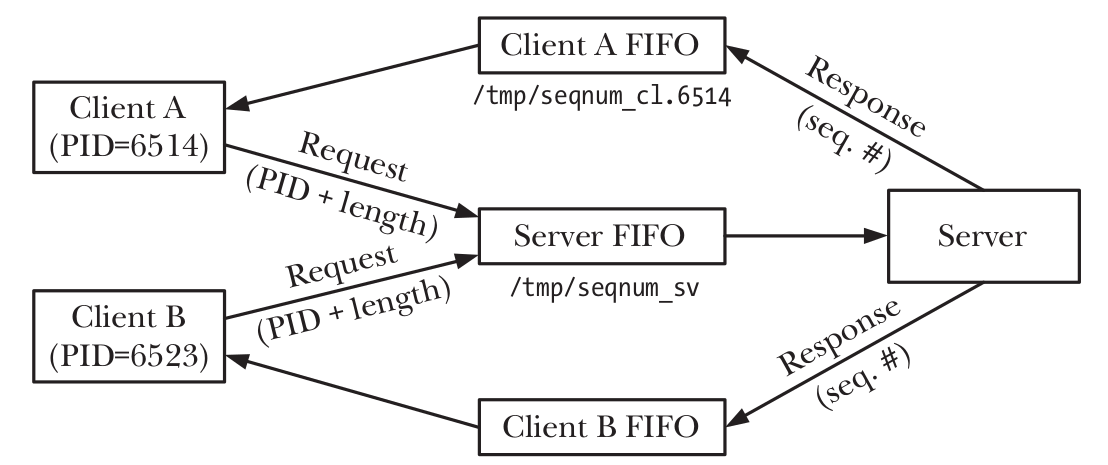
\includegraphics[width=.7\textwidth]{fifo-client-server.png} % size, path
	\caption{Fifo client-server model}
	\label{fig:fifocs}
\end{figure}

\vspace{2mm} 
Na Slici \ref{fig:fifocs} prikazan je client-server model komunikacije putem \texttt{fifo-a}.

Potrebno je uvesti i konvenciju po kojoj će se određivati dužina poruke koju \texttt{client} tj. \texttt{server} proces prima. Postoji više mogućih načina da se ovo realizuje, navešćemo neke od njih:

\begin{enumerate}[1)]
	\item{\texttt{delimiter character} --- Poruke se razdvajaju nekim karakterom, npr. \texttt{'\textbackslash n'}.}
	\item{\texttt{fixed-length} --- Poruke su unapred određene fiksne dužine.}
	\item{\texttt{fixed-size header} --- Svaka poruka ima header fiksne dužine u kome je navedena dužina poruke.}
\end{enumerate}

\newpage

U primerima \ref{lst:fifoserver} i \ref{lst:fifoclient} prikazana je moguća implementacija \texttt{client-server} modela, u kome se poruke sa \texttt{standardnog ulaza} servera prosleđuju na \texttt{standardni izlaz} klijenta.

\vspace{2mm} 
\scode{fifo_server.c}{Fifo server}{fifoserver}

\scode{fifo_client.c}{Fifo klijent}{fifoclient}
\stdio{Standardni ulaz fifo servera}{Standardni izlaz fifo klijenta}{Write in C \\ Hello World \\ kraj}{Write in C \\ Hello World}
\vspace{2mm} 

Dati primer \texttt{FIFO} \texttt{client-server} komunikacije koristi \texttt{delimiter character} metod za razdvajanje poruka, taj karakter je \texttt{'\textbackslash0'} tj. terminalna nula, što omogućava udobnu komunikaciju pomoću string-ova. 

\newpage

\subsection{Deljena memorija}
Procesi često imaju potrebu da pristupaju zajedničkoj memoriji, tj. da čitaju iz nje, pišu u nju. 
Da bi bili u mogućnosti da je koriste potreban im je način za kreiranje i način za pristupanje toj deljenoj memoriji. U \texttt{Linux} okruženju postoje funkcije koje se bave ovom problematikom.

\begin{figure}[h]
	\centering
	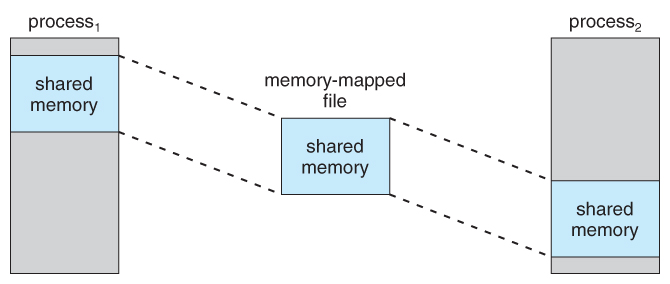
\includegraphics[width=.7\textwidth]{shm.jpg} % size, path
	\caption{Deljenje memorije}
	\label{fig:shm}
\end{figure}

Deljena memorija predstavlja fajl u \texttt{linux fajl sistemu} koji sadrži podatke (memoriju). Tu memoriju možemo potom možemo mapirati u adresni prostor programa. 

\begin{center}
	\texttt{int shm\_open(const char * name, int oflag, mode\_t mode);} \\
	\texttt{int shm\_unlink(const char * name, int oflag, mode\_t mode);}
\end{center}
\textbf{Povratna vrednost:} \texttt{shm\_open()} u slučaju uspeha vraća fajl deskriptor, \texttt{-1} u slučaju greške. \texttt{shm\_unlink()} u slučaju uspeha vraća 0, u suprotnom \texttt{-1}.

Za kreiranje/pristup deljenoj memoriji koristimo funkciju \texttt{shm\_open()} i to: 
\vspace{-2mm} 
\begin{enumerate}[1)]
	\item{Za kreiranje: \texttt{shm\_open(naziv, O\_RDWR | O\_CREAT, 0755);}}
	\item{Za otvaranje: \texttt{shm\_open(naziv, O\_RDWR, 0);}}
	\item{Za brisanje: \texttt{shm\_unlink(naziv);}}
\end{enumerate}
\vspace{-1mm} 

Kada otvorimo deljenu memoriju, potrebno ju je još i mapirati u adresni prostor.

\begin{center}
	\texttt{void *mmap(void *addr, size\_t len, int prot, int flags, int fildes, off\_t off);} \\
	\texttt{int munmap(void *addr, size\_t length);}
\end{center}

Prvi argument nam nije potreban i njega ćemo zanemariti, tj. prosledićemo \texttt{NULL}, drugi argument predstavlja veličinu memorije, treći su prava pristupa (\texttt{PROT\_READ, PROT\_WRITE}). Argument \texttt{flags} je tip memorije koji alociramo, najčešće ćemo koristiti \texttt{MAP\_SHARED}. Zatim ide fajl deskriptor deljene memorije, i na kraju ofset od početka fajla. \texttt{munmap()} ``unmapira" memoriju. Od argumenata prima adresu i dužinu memorije. 

\textbf{Povratna vrednost:} \texttt{mmap()} u slučaju uspeha vraća adresu mapirane memorije, u slučaju greške vraća \texttt{MAP\_FAILED}. \texttt{munmap()} vraća \texttt{0}, a u slučaju greške \texttt{-1}.

\vspace{2mm} 
\textbf{NAPOMENA:} Kada kompiliramo program koji koristi funkcije koje rade sa deljenom memorijom, potrebno je navesti i argument -lrt. 

 \begin{center}
	\texttt{gcc shm.c -o shm -std=c99 -Wall -Wextra -lrt} 
\end{center}
\newpage
\subsubsection{Primeri deljenja memorije}

Dati su primeri kreiranja deljenja memorije (Primer \ref{lst:shmcr}) i čitanja iz deljene memorije (Primer \ref{lst:shmget} na strani \pageref{lst:shmget}). Prvo se pokreće program iz primera \ref{lst:shmcr} a nakon njegovog uspečnog izvršavanja pokreće se i program \ref{lst:shmget}. Program koji kreira deljenu memoriju učitava niz sa \texttt{standardnog ulaza} u deljenu memoriju, a program koji otvara deljenu memoriju ispisuje taj niz na \texttt{standardni izlaz}. \texttt{\_shared\_array } je struktura koja nam olakšava razmenu podataka.
\vspace{2mm} 

\scode{shmcreate.c}{Kreiranje deljene memorije}{shmcr}

\vspace{5mm} 
Program iz primera \ref{lst:shmcr} čita niz sa \texttt{standardnog ulaza} i upisuje ga u \texttt{deljenu memoriju}.

\newpage
Program iz primera \ref{lst:shmget} čita niz iz deljene memorije i ispisuje ga na \texttt{standardni izlaz.} 
\vspace{1mm} 

\scode{shmget.c}{Otvaranje deljene memorije}{shmget}
\stdio{Ulaz programa iz primera \ref{lst:shmcr}}{Izlaz programa iz primera \ref{lst:shmget}}{5\\ 1.22 2.51 3.14 2.72 1.81}{1.22 2.51 3.14 2.72 1.81}

\vspace{2mm} 
Primetimo da ovaj program ima jedan nedostatak, istovremeno pokretanje oba programa može dovesti do problema. Na ovaj primer ćemo se vratiti kada budemo izučavali neke od metoda sinhronizacje.

\newpage
\subsection{Semafori}

Semafori obezbeđuju sinhronizaciju između procesa (često radi pristupanja deljenoj memoriji). Semafor je struktura koja ima svoju vrednost (celobrijnu promenljivu tipa \texttt{sem\_t}) i skup operacija koje se mogu izvršiti nad njom, te operacije su: 
\vspace{-2mm} 

\begin{enumerate}[1)]
		 \item{Uvećanje trenutne vrednost semafora.}
		 \item{Umanjenje trenutne vrednosti semafora.}
		 \item{Čekanje da vrednost semafora postane 0}
		 \item{Postavljanje vrednosti semafora na njenu apsolutnu vrednost.}
\end{enumerate}


Kada kreiramo semafor, pre nego što počnemo da ga koristimo potrebno je inicijalizovati ga na određenu vrednost. Ta vrednost predstavlja broj \texttt{procesa/threadova} koji mogu pristupiti resursu koji semafor ``štiti". Kada je vrednost semafora \texttt{0} onda je resurs dostupan. Promenljiva tipa \texttt{sem\_t} tj. semafor treba biti vidljiv svim procesima/threadovima koji ga koriste (npr. globalna promenljiva ili statički alocirana promenljiva koju možemo proslediti kao argument). 

Funkcije pomoću kojih su ove operacije realizovane su:

\hspace{.17\textwidth} 
\begin{minipage}[t]{.66\textwidth} % Width (ex. .475)
\begin{veratim}
	\texttt{int sem\_init(sem\_t *sem, int pshared, int value);} \\
	\texttt{int sem\_wait(sem\_t *sem);} \\
	\texttt{int sem\_post(sem\_t *sem);} 
\end{verbatim}
\end{minipage}
\vspace{2mm} 

\texttt{sem\_init()} --- Inicijalizuje semafor čiji se pokazivač prosleđuje kao prvi argument, drugi argument određuje da li će semafor biti deljen između procesa (1) ili izmedju threadova jednog procesa (0). Treći argument je vrednost na koju se inicijalizuje. \\
	\texttt{sem\_wait()} --- Umanjuje vrednost semafora za \texttt{1} i pristupa resursu ili čeka ukoliko je resurs zauzet (ukoliko je vrednost semafora \texttt{0}). \\
	\texttt{sem\_post()} --- Uvećava vrednost semafora za \texttt{1} i signalizira mogućnost neke operacije koja sledi i sl.

\textbf{Povratne vrednosti:} \texttt{0}  u slučaju uspešnog izvršavanja, u slučaju greške \texttt{-1} i \texttt{errno} promenljiva je postavljena na odgovarajuću vrednost.

Vrednost semafora najčešće stavljamo zajedno za podacima, što omogućava udobnije korišćenje semafora.

\scode{structsem.c}{Struktura koja sadrži semafore}{semstruct}


\vspace{2mm} 
 \textbf{NAPOMENA:} Kada kompiliramo program koji koristi funkcije koje rade sa semaforima, potrebno je navesti i argument -lpthread. 

\begin{center}
	\texttt{gcc sem.c -o sem -std=c99 -Wall -Wextra -lpthread} 
\end{center}



\newpage

Primeri \ref{lst:semwr} i \ref{lst:semrd} predstavljaju modifikacije  primera \ref{lst:shmcr} i \ref{lst:shmget} koji nisu koristili nikakvu sinhronizaciju, dok novi primeri koriste sinhronizaciju putem semafora. Ulazne i izlazne vrednosti ostaju nepromenjene, ali je ipak uklonjena mogućnost bilo kakvog nedeterminističkog ponašanja.

\scode{sem_shm_writer.c}{Modifikacija primera \ref{lst:shmcr}}{semwr}

\scode{sem_shm_reader.c}{Modifikacija primera \ref{lst:shmget}}{semrd}

\subsection{Zaključavanje fajlova}

Dok jedan proces pristupa fajlu, neće doći do problema prilikom čitanja tj. pisanja u taj fajl. Ali kada više procesa pristupa istom fajlu, dolazi do tzv. trke za resursima. Da bismo rešili taj problem treba nam opet neka vrsta sinhronizacije. U linux okruženju imamo određene sistemske pozive koji se bave ovom problematikom.

Kod zaključavanja fajla (postavljanja katanca) imamo dve operacije: 
\vspace{-2mm} 
\begin{enumerate}[1)]
	\item{\texttt{acquire} --- Postavlja katanac na fajl/njegov deo}
	\item{\texttt{release} --- Skida katanac sa fajla/dela}.
\end{enumerate}

Ove se realizuju prosledjivanjem argumenata odgovarajućih argumenata \texttt{fcntl()} sistemskom pozivu.


\hspace{.17\textwidth} 
\begin{minipage}[t]{.66\textwidth} % Width (ex. .475)
	\begin{veratim}
		\texttt{int fcntl(int fd, int cmd, ... /* arg */ );}
	\end{verbatim}
\end{minipage}
\vspace{2mm} 

\textbf{Povratna vrednost:} Zavisi od tipa poziva, tj. argumenata koje smo prosledili. U slučaju greške je \texttt{-1} i \texttt{errno} promenljiva se postavlja na odgovarajuću vrednost.

\vspace{2mm} 

\texttt{fcntl()} sistemski poziv izvršava neku od operacija nad fajlom koji je prosleđen putem fajl deskriptora kao što su dupliranje fajl deskriptora, promena vrednosti fajl deskriptora i slično. Između ostalog uz pomoć ovog sistemskog poziva mogu se staviti i tzv. katanci koji onemogućuju drugim procesima da manipulišu podacima u datom fajlu. 

\vspace{1mm} 
Katanci \texttt{fcntl()} sistemskog poziva su katanci za sinhronizaciju, oni neće onemogućiti nekome da piše/čita iz fajla sem ukoliko želi sinhronizaciju i sam proveri da li postoje katanci. Dakle ova vrsta zaključavanja neće onemogućiti nekog ko ima jaku nameru da pristupi našem fajlu, već ga može obavestiti: ``Hej, ovaj segment fajla je zaključan.". Na tom principu rade katanci sistemskh poziva \texttt{fcntl()} i \texttt{flock()}.

Zaključavanje se vrši tako što se kao drgi argument prosledi \texttt{F\_SETLK} i kao treći struktura tipa \texttt{struct flock} čiji član strukture (promenljiva) \texttt{l\_type} određuje tip katanca npr(\texttt{F\_WRLCK ili F\_RDLCK)}.

Za otključavanje drugi argument je takođe F\_SETLK, a tip katanca \texttt{l\_type} treba da bude \texttt{F\_UNLCK}.

\vspace{2mm} 
\scode{struct_flock.c}{Struktura flock}{structflock}
\vspace{4mm} 

Struktura \texttt{flock} data u primeru \ref{lst:structflock} korišćena je u primeru \ref{lst:flock} na strani \pageref{lst:flock} kod postavljanja katanca u fajlu (zaključavanja).
 
\newpage

U Primeru \ref{lst:flock} na \texttt{standardni ulaz} se prosleđuju ime fajla, od kog bajta ga treba zaključati i vreme trajanja katanca. Katanac biva zadržan na traženom delu fajla onoliko sekundi koliko smo uneli sa standardnog ulaza (sačuvali u promenljivu \texttt{lock\_time}).

\vspace{2mm} 
\scode{flock.c}{Zaključavanje fajla}{flock}
\stdio{Standardni ulaz:}{Standardni izlaz:}{\texttt{file.txt 10 30 20}}{\texttt{Enter: fpath from len lock\_time\\Lock acquired, holding 20 seconds.\\ Lock released ...}}

\vspace{3mm} 
Dodatne informacije o zaključavanju fajlova potražite u: \texttt{man 2 fcntl}.

\newpage

\subsection{Rad sa nitima}

Niti nam obezbeđuju mogućnost da se u okviru jednog procesa izvršava više radnji istovremeno (svaka nit posebnu radnju). Niti dele deskriptore i memoriju procesa u okviru koga su pokrenute. Sinhronizacija prilikom korišćenja niti može biti značajno jednostavnija nego između procesa, a značajno je i to što na višeprocesorskim sistemima dobijamo poboljšane performanse.
\vspace{3mm} 

\begin{figure}[h]
	\centering
	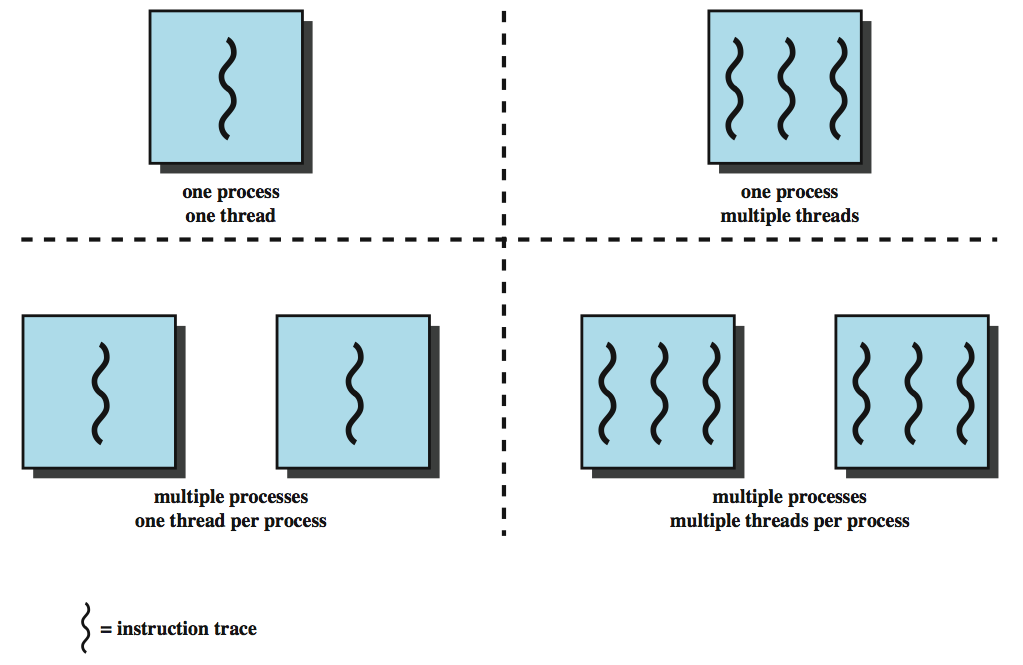
\includegraphics[width=.7\textwidth]{./img/mthread.png} % size, path
	\vspace{-2mm} 
	\caption{Izvršavanje više niti istovremeno}
	\label{fig:mthread}
\end{figure}

\scode{mutex_func.c}{Funkcije za rad sa threadovima}{fthreads}	

\vspace{5mm} 
Greške kod funkcija datih u Primeru \ref{lst:fthreads} treba obrađivati funkcijom \texttt{pth\_check()} koju možete videti u Primeru \ref{lst:obrg} na strani \pageref{lst:obrg}.
\vspace{1mm} 
\newpage

U Primeru \ref{lst:simplenit} možemo videti jedostavno kreiranje i izvršavanje niti. Funkciju korišćenu za obradu greške (\texttt{pth\_check()} možete naći u Primeru \ref{lst:obrg} na strani \ref{lst:obrg}.

\scode{simplethr.c}{Kreiranje niti}{simplenit}
\stdio{Standarni ulaz:}{Standardni izlaz:}{}{\texttt{Stampam iz prve niti. \\ Stampam iz druge niti}}

\textbf{NAPOMENA:} Kada kompiliramo program koji koristi funkcije koje rade sa posix threadovima, potrebno je navesti i argument -lpthread. 

\begin{center}
	\texttt{gcc pthreads.c -o pthreads -std=c99 -Wall -Wextra -lpthread} 
\end{center}

\newpage

U Primeru \ref{lst:visenitniprog} možemo videti na koji način se mogu kreirati niti, kako im se prosleđuju argumeni kao i uzimanje povratne vrednosti iz funkcije niti. Promenljiva \texttt{static double retval} živi od početka do kraja programa a vidljivost ima na nivou funkcije. Potrebno je pozivanje funkcije \texttt{thr3()} da bi uzela vrednost \texttt{2.72}, inače bi bila \texttt{3.14}.

\scode{thr_create.c}{Izvršavanje programa sa vise niti}{visenitniprog}
\stdio{Standarni ulaz:}{Standardni izlaz}{\texttt{Zdravo svete} }{\texttt{Unesite 2 stringa (argumente niti):\\ Treca nit, string je: svete \\ Druga nit, string je: Zdravo \\ Povratna vrednost thr3: 2.72}}

Primetimo da pri izvršavanju datog programa ne možemo reći koja nit će se pre izvršiti (nit2 ili nit3). Ukoliko nam je redosled izvršavanja bitan, morali bismo da pozovemo funkciju \texttt{pthread\_join()} nakon kreiranja druge niti a pre kreiranja treće tako bismo ovezbedili izvršavaju u redosledu nit2, nit3.

\subsection{Mutual exclusion (mutex)}

Proces ima više niti, te niti se mogu izvršavati paralelno. Ukoliko niti imaju porebu da menjaju zajedničke resurse npr. globalnu promenljivoj itd. može doći do problema u sinhronizaciju. Za sinhronizaciju niti koristimo \texttt{mutex-e} (Mutual exclusion).

Mutex-ima ograničavamo tzv. kritične delove koda, npr. deo koda u kome se izmenjuje neki deljeni resurs. Kada nit zaključa \texttt{mutex}, bilo koja druga nit koja pokša da ga zaključa biće blokirana, tako isto i sledeća itd. Sve dok se prvi \texttt{mutex} ne otključa, pa drugi itd.

\vspace{2mm} 
\scode{mutex_lock.c}{Funkcije za rad sa mutex-ima}{mutfunc}

\vspace{2mm} 
 \textbf{NAPOMENA:} Kada kompiliramo program koji koristi funkcije koje rade sa mutex-ima, potrebno je navesti i argument -lpthread. 
 \vspace{2mm} 

\begin{center}
	\texttt{gcc mutex.c -o mutex -std=c99 -Wall -Wextra -lpthread} 
\end{center}

\newpage
\section{Korisne stvari}

\subsection{Čitanje liniju po liniju}

Funkcija \texttt{getline()} čita liniju sa iz toka \texttt{stream-a}, to može biti standardni ulaz npr.
\begin{center}
	\texttt{ssize\_t getline(char **lineptr, size\_t *n, FILE *stream);}
\end{center}

Funkcija \texttt{getdelim()} radi isto što i \texttt{getline()} ali delimiter karakter se prosleđuje (zamenjuje '\textbackslash n').

\begin{center}
	\texttt{ssize\_t getdelim(char **lineptr, size\_t *n, int delim, FILE *stream);}
\end{center}

\textbf{Povratna vrednost:} Broj pročitanih bajtova uključujući i \texttt{delimiter} karakter, ali be \texttt{'\textbackslash 0'} karaktera u slučaju uspeha. -1 u slučaju neuspešnog čitanja i \texttt{errno} se postavlja na odgovarajuću vrednost.

\scode{getline.c}{Čistanje liniju po liniju sa stdout}{getline}

\subsection{Saveti za ispit}

\begin{itemize}
	\item{Možete pretražiti sve man strane komandom: \\ \vspace{-3mm} \begin{center}\texttt{man -k . | grep KLJUCNA\_REC}\end{center}}
			\vspace{1mm} 
	\item{Možete pretražiti man strane sistemskih poziva komandom: \\ \vspace{-3mm} \begin{center}\texttt{man -2 syscalls | grep KLJUCNA\_REC}\end{center}}
			\vspace{1mm} 
		\item{Ukoliko ste uključili sva potrebna zaglavlja a kaze vam da funkcija nije definisana, postoji velika mogucnost da ste zaboravil neku definiciju tipa: \\ \vspace{-3mm} \begin{center}\texttt{\#define \_GNU\_SOURCE (500)}\end{center}}
			\vspace{1mm} 
	\item{Kompilirajte kod tako da vam pokazuje sve moguće greške i upozorenja: \\ \vspace{-3mm} \begin{center}\texttt{gcc primer.c -o primer -std=c99 -Wall -Wextra}\end{center}}
			\vspace{1mm} 
	\item{Proverite povratnu vrednost u slučaju uspeha/greške komandom \texttt{shell-a}: \\ \vspace{-3mm} \begin{center}\texttt{echo \$?}\end{center}}
			\vspace{1mm} 
	\item{Ukoliko vam se javlja greška u fazi linkovanja, verovatno ste zaboravili da kompajleru navedete biblioteku koja se dinamičk povezuje: \\ \vspace{-3mm} \begin{center}\texttt{gcc primer.c -o primer-lpthread -lrt -lm -lNESTO}\end{center}}
			\vspace{1mm} 
		\item{Ponekad se mogu iskoristiti primeri koji se nalaze u man stranama.}
			\vspace{1mm} 
			\item{Budite pažljivi prilikom obrade grešaka}
\end{itemize}

\end{document}
